\section{Versuchsaufbau}
    \begin{figure}[ht]
        \centering
        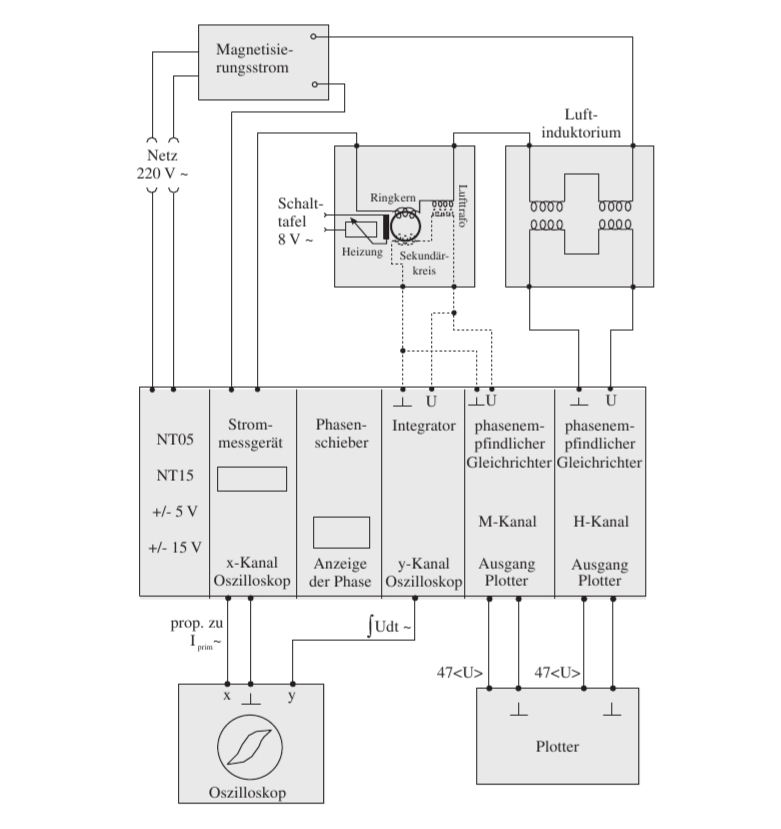
\includegraphics[width=\textwidth]{Images/Schaltplan.PNG}
        \label{Schaltplan}
        \caption{Schaltplan des Versuchs}
    \end{figure}
    Um in diesem Versuch möglichst viele Parameter variieren zu können werden zwei verschiedene Versuchsaufbauten verwendet.

    \subsubsection*{Ringkern mit Heizung}
        Bei diesem Aufbau handelt es sich um einen geschlossenen Ferrit Ringkern mit Heizspule um den Temperaturverlauf aufzeichnen zu können.\\
        Primär- und Sekundärspule haben jeweils $n=17$ Windungen, der Ringkern hat einen Querschnitt von $q=0,9cm^2$ und einen Radius von $r=1.5cm$.
        Die Heizgeschwindigkeit lässt sich über ein Potentiometer regulieren und mit Hilfe eines Thermoelements messen.
    
    \subsection*{Ringkern mit Spalt}
        Um nun im Ringkern einen Spalt zu erzeugen lässt sich dieser Aufbau auseinanderziehen und mit Plättchen variierender Dicke auf vorgegebenen Abständen halten.
        In diesem Aufbau hatte die Primärspule hingegen $n_p=54$ und die Sekundärspule $n_s=17$ Windungen\\
        
    Bei beiden aufbauten wurde, um den Einfluss der Umgebung zu eliminieren, je ein Luftinduktor in Reihe geschaltet. Die Messausgänge der Gesamtschaltung (siehe \ref{Schaltplan}) konnten 
    dabei je nach Messung zwischen den Eingängen des Oszilloskops und der Gleichrichter gewechselt werden.